\documentclass[onecolumn,showpacs,preprintnumbers,prl,amsmath,amssymb]{revtex4-1}

\def\b{\mathbf}
\def\e{\epsilon}

\usepackage{graphicx}% Include Fig.~files
\usepackage{dcolumn}% Align table columns on decimal point
\usepackage{bm}% bold math
\usepackage{color}


\begin{document}


\title{Unstable active networks}

\author{Devin Kachan$^1$}
\author{Arthur A. Evans$^2$}
 

\affiliation{$^1$ Department of Physics, University of California Los Angeles,\\ 405 Hilgard Ave, Los Angeles CA 90095.}

\affiliation{$^2$ Department of Chemistry and Biochemistry, University of California Los Angeles,\\ 405 Hilgard Ave, Los Angeles CA 90095.}


\date{\today}

\begin{abstract}
Active gels: do THEY buckle?
\end{abstract}

\maketitle


%%%%%%%%%%%%%%%%%%%%%
\section{Introduction}

\section{Kinetic equation for motors}

Imagine that we have a gel of actin filaments immersed in a solvent, and surrounded also with number of molecular motors (dyne in, kinesin, etc.). These motors have a certain probability to bind to the filaments and exert stresses, meaning the the whole system has the potential to have local stresses that obey nematic order. We write a Smoluchowski equation for the 1-particle distribution function $\psi$ of bound motors:

\begin{gather}
\frac{\partial \psi}{\partial t}+\nabla\cdot(\dot{\b{x}}\psi)=k_{on}\psi^{*}-k_{off}e^{-|\sigma|/\sigma_0}\psi,
\end{gather}
where $\sigma$ is the absolute value of the stress in the medium, to be determined by stress balance, and $\b{x}$ is the local position of the motor distribution. $\sigma_0$ is a scale that determines how much stress is required to enhance the binding affinity of the motors.  If the displacement field of the underlying gel can be described with a displacement field $\b{u}$, the no-slip condition between the bound motors and the filaments ensures that $\dot{\b{x}}=\partial \b{u}/\partial t$. Momentum conservation ensures that the (visco)elastic stress caused by the displacement must be balanced by the active stress $\b{\Sigma}$ caused by the motors:

\begin{gather}
\nabla\cdot\b{\sigma}=-\nabla\cdot\b{\Sigma}.
\end{gather}

The active stress $\b{\Sigma}=\alpha \b{Q}\psi$, where $\b{Q}$ is the nematic order parameter of the filaments. If we consider the over-damped limit, or, equivalently, the homogeneous limit, then we get the following reduced equation for the evolution of the bound concentration:

\begin{gather}
\frac{\partial\psi}{\partial t}=A-Be^{-\beta \psi}\psi,
\end{gather}
where $\beta=(\alpha/\sigma_0) \sqrt{Q_{ij}Q^{ij}}$ (or something) and $A,B$ are the respective reaction coefficients. We can make some attempt to quantify the stability of this solution by examining the fixed points, i.e. $\bar{\psi}$ such that $B\bar{\psi}e^{-\beta\bar{\psi}}=A$. This is actually the definition of the Lambert function $W(z)$, defined implicitly by the relationship $z=W(z)e^{W(z)}$ for any complex number $z$. The condition for a fixed point for our motor concentration is then given by

\begin{gather}
\bar{\psi}=-\frac{1}{\beta}W\left(-\frac{A\beta}{B}\right).
\end{gather}
A contour plot is shown in figure \ref{contour}, measuring $\bar{\psi}$ as a function of $\beta$ and the reduced reaction coefficient $\mu=A/B$. The white region has no purely real solution, indicating that no fixed point exists, and the motor concentration grows without bound.

Since the Lambert W function is multivalued on the open set $(-1/e,0)$, we expect that there will be two fixed points for appropriate parameter values. We know that the principal branch $W_0(z)$ has the value $W_0(-1/e)=-1$, and thus we can solve for the critical value of $\beta$ beyond which there can be no fixed point, i.e. $\beta^*=1/\mu e$.

In figure \ref{fixedpts} we plot the fixed points of the system. Note that above $\beta^*$ there are no fixed points, while even below this critical value there is an unstable fixed point. The basin of stability for the system is then bounded by the two curves shown in figure \ref{fixedpts}, and we can estimate the parameter values that will lead to instability.

\begin{figure}
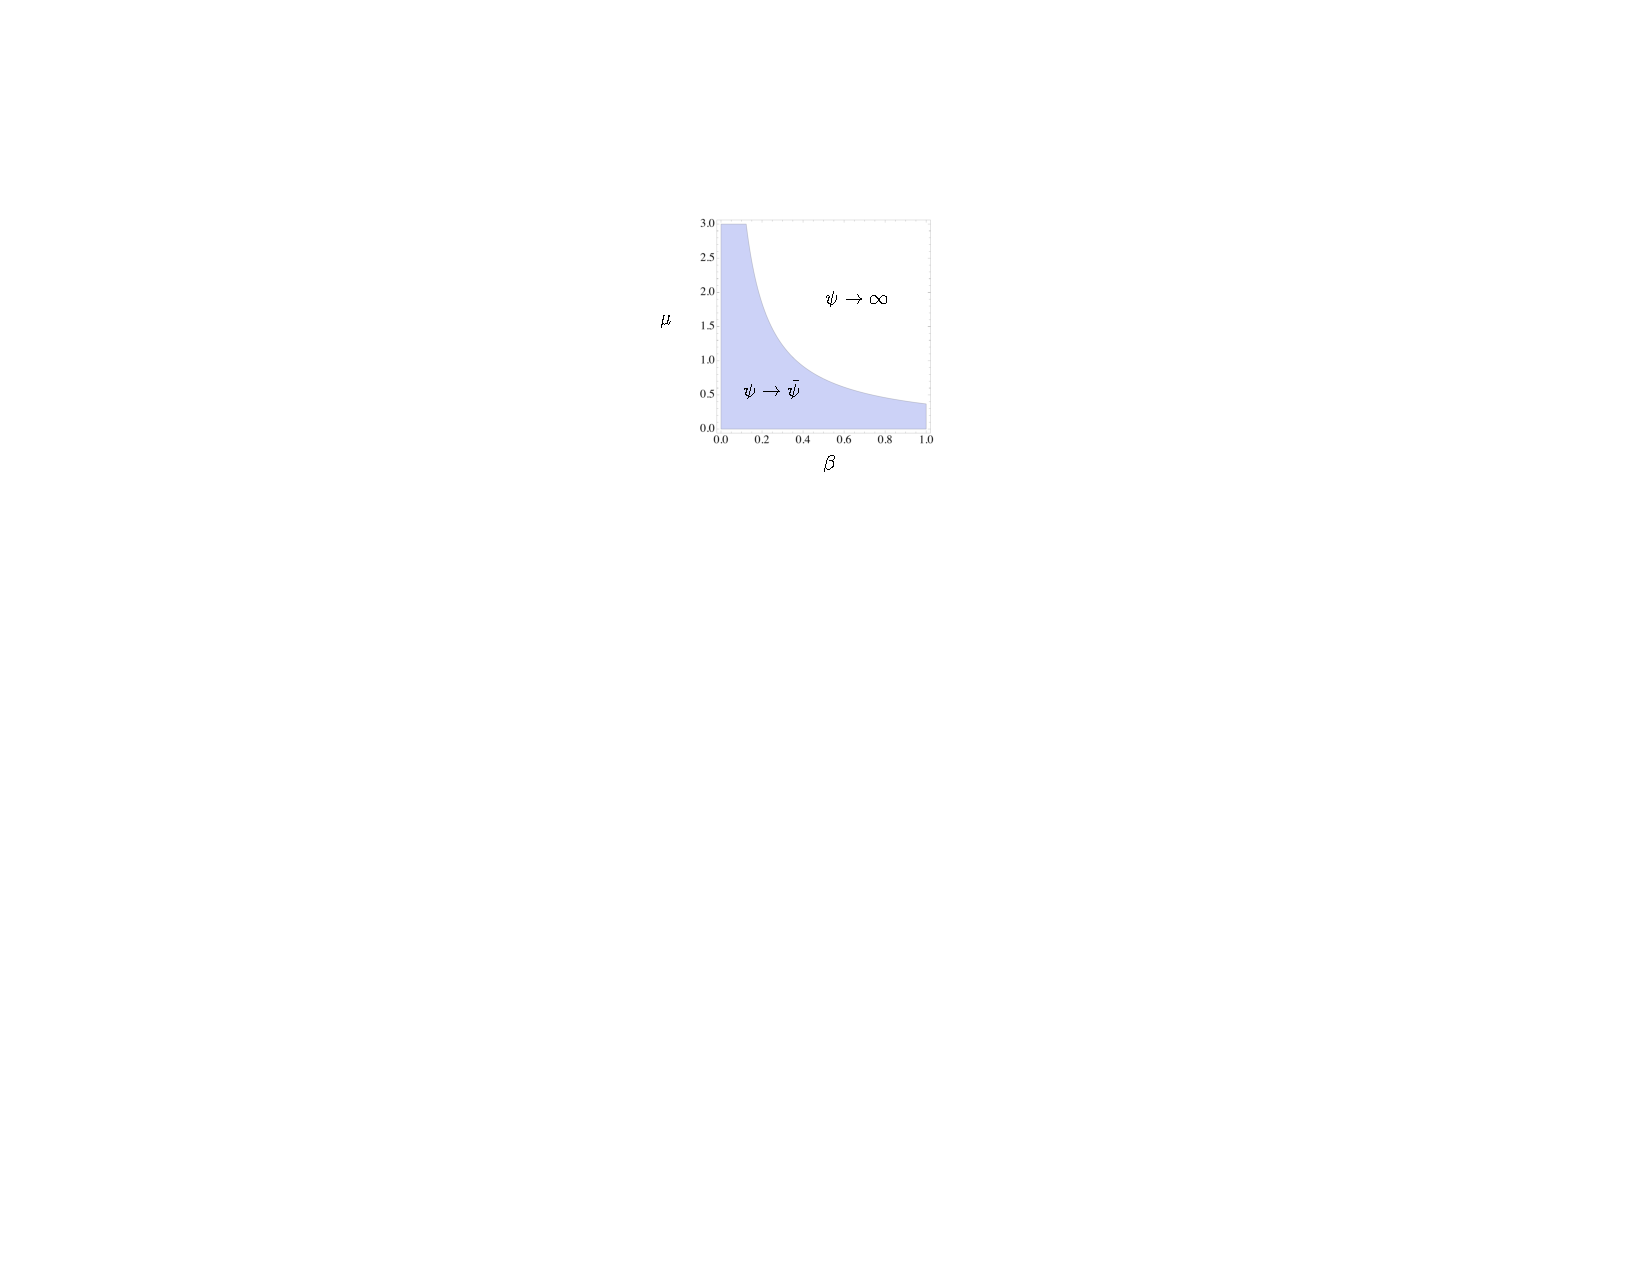
\includegraphics[width=.75\textwidth] {fig1}
\caption{\label{contour} Contour plot show the region of stability for the reduced model of bound motor concentration. For large $\mu$ the chemical potential between the solution and bound motors is such that any amount of order will destabilize the system. Alternatively, for large enough pulling force or ordering (i.e. large $\beta$), even a small $\mu$ leads to destabilization.  }
\end{figure}

\begin{figure}
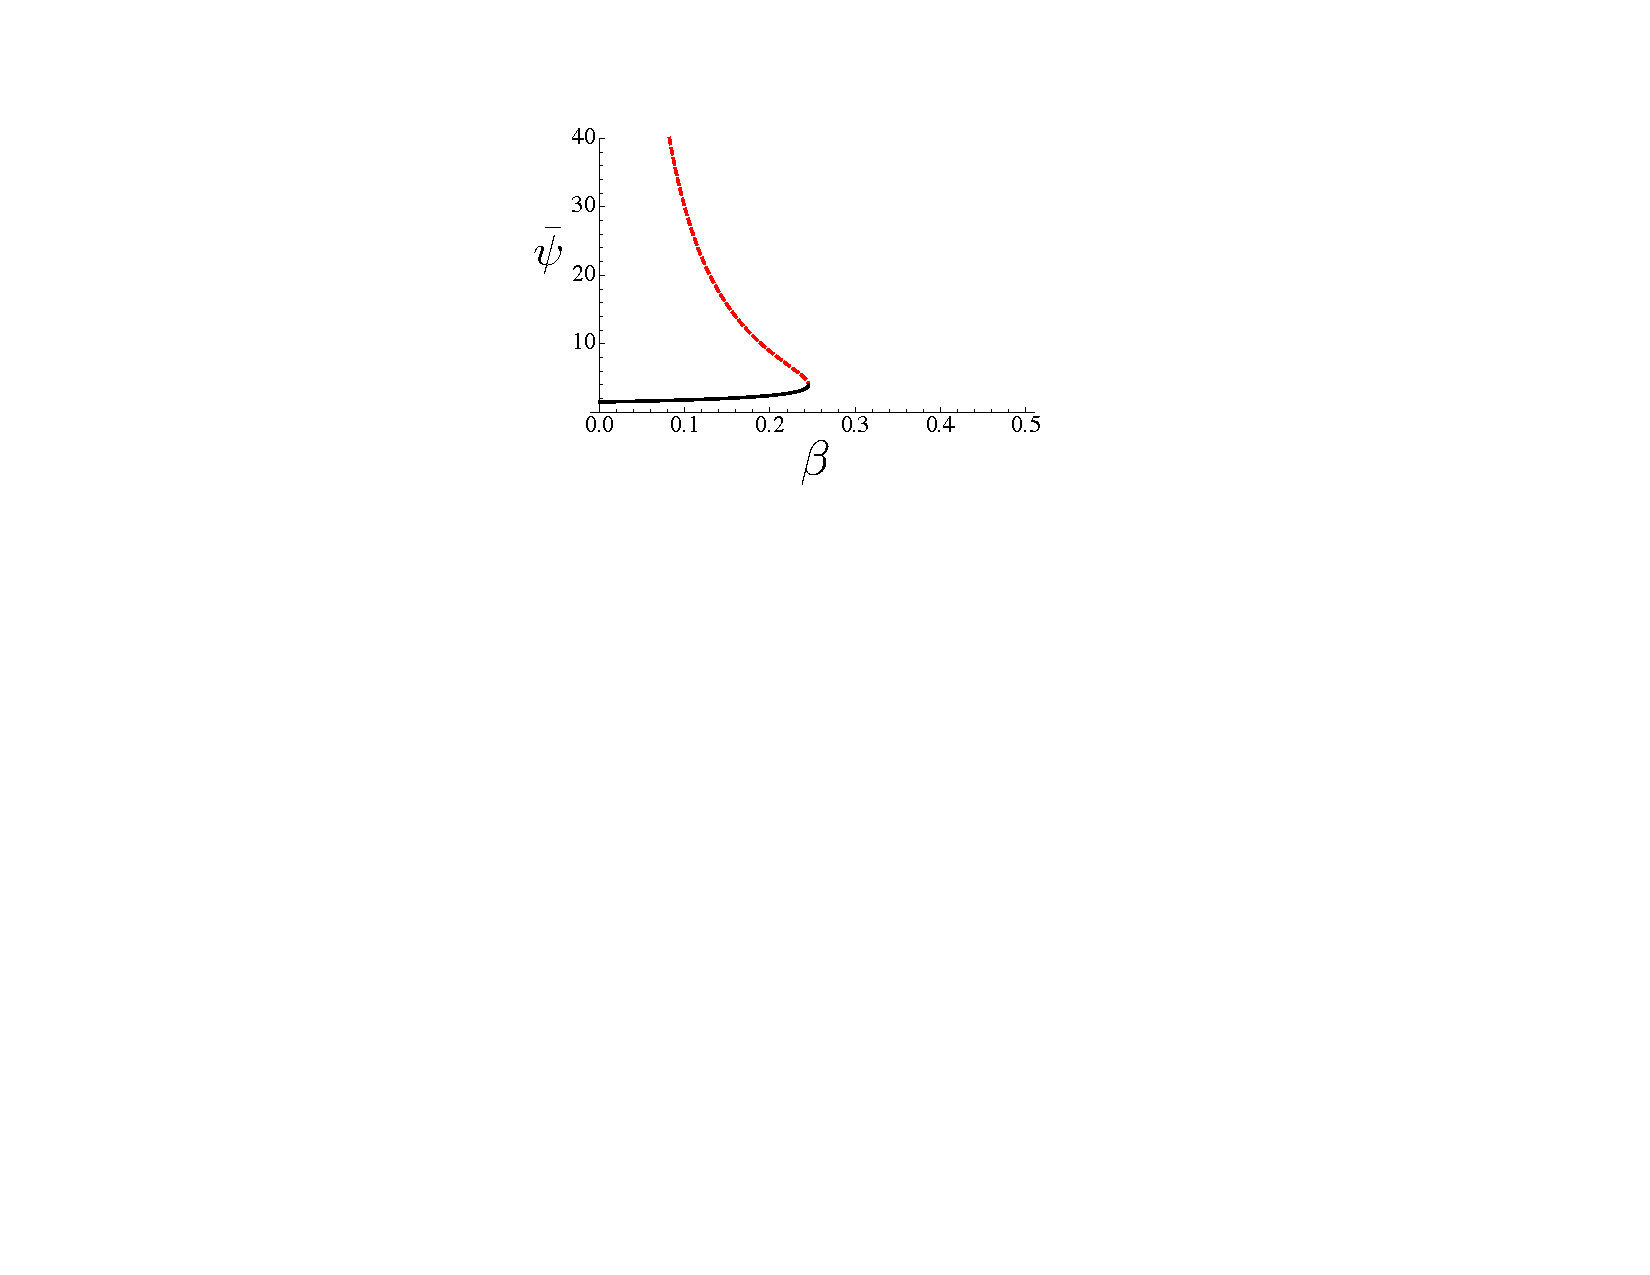
\includegraphics[width=.75\textwidth] {fig2}
\caption{\label{fixedpts} Fixed points for the minimal active gel system, for $\mu=1.5$. The red (dashed) line corresponds to the unstable fixed point, while the black (solid) line is stable. Both disappear in a ``blue sky" bifurcation above the critical value of $\beta^*=1/\mu e$. Mathematically, these two fixed points correspond to the principal $W_0(-\mu\beta)$ branch (stable fixed point) and the lower branch $W_{-1}(-\mu\beta)$.}
\end{figure}

\section{Spatio-temporal evolution}

This is slightly more complicated if we allow for spatial dependence, and consider that the displacement field can vary in time. In this case we would then have

\begin{gather}
\frac{\partial \psi}{\partial t}+\nabla\cdot\left(\frac{\partial\b{u}}{\partial t}\psi\right)=k_{on}\psi^{*}-k_{off}e^{-|\sigma|/\sigma_0}\psi,\\
\frac{\partial \b{u}}{\partial t}=-\nabla\cdot\sigma-\nabla\cdot\b{\Sigma}.
\end{gather}

Probably the only thing that we can do here is linearize and examine whether or not any particular wavelengths are selected as the most unstable. If we develop the variables $\psi, \b{u}, \sigma $ in a perturbation series $\sigma=\epsilon\sigma^{(0)}+\epsilon^2\sigma^{(1)}+...$, $\psi=\psi^{(0)}+\epsilon\psi^{(1)}+...$, etc. where $\epsilon$ is a measure of homogeneity of the system, then perhaps we can make some sort of progress. To $O(\epsilon^0)$ we have

\begin{gather}
\partial_t\psi^{(0)}=k_{on}\psi^*-k_{off}\psi^{(0)}\\
\alpha\nabla\cdot(\b{Q}\psi^{(0)})=0.
\end{gather}
This results from assuming that the stress and displacement are formally lower order than the concentration. Can we do that? I don't know, but I did.

To $O(\epsilon)$

\begin{gather}
\frac{\partial \psi^{(1)}}{\partial t}+\nabla\cdot\left(\frac{\partial\b{u}^{(0)}}{\partial t}\psi^{(0)}\right)=k_{on}\psi^{*}+k_{off}\psi^{(1)}-k_{off}\frac{\sigma^{(0)}}{\sigma_0}\psi^{(0)},\\
\frac{\partial \b{u}^{(0)}}{\partial t}=-\nabla\cdot\sigma^{(0)}-\alpha\nabla\cdot\left(\b{Q}\psi^{(1)}\right).
\end{gather}


\section{Active suspensions: a review}

The kinetic theory describing the hydrodynamics of a dilute suspension of active spheroidal particles begins with a distribution function $\psi(\b{r},\b{p},t)$ that satisfies the following Smoluchowski equation:

\begin{gather}
\label{eq:Smoluchowski}
\partial_t\psi+\nabla_x\cdot(\b{\dot{x}}\psi)+\nabla_p\cdot(\b{\dot{p}}\psi)=0,
\end{gather}
where $\nabla_p=(\b{I}-\b{pp})\cdot\partial_p$ is the gradient acting on the unit sphere. This Smoluchowski equation enforces the conservation of particles. Note that conservation equations of this form are effectively derived from the BBGKY hierarchy, through the Boltzmann equation; when we add correlations or ``collisions"  we will have to recall where our distribution function came from in order to make sure everything that we add makes sense.

For motile rodlike particles we have the following equations governing the dynamics of the rotation and center of mass:

\begin{gather}
\b{\dot{x}}=V\b{p}+\b{u}-D\nabla_x\log\psi,\\
\b{\dot{p}}=(\b{I}-\b{pp})\cdot\left[\gamma\b{E}+\b{W}\right]\cdot\b{p}-D_R\nabla_p\log\psi
\end{gather}
Here $V$ is the self-propulsion velocity (if any), $\b{u}$ is the fluid velocity of the solvent, $D$ and $D_R$ are diffusion constants, $2\b{E}=\nabla_x\b{u}+\nabla_x\b{u}^T$ is the symmetric rate of strain tensor, while $2\b{W}=\nabla_x\b{u}-\nabla_x\b{u}^T$ is the vorticity tensor. The parameter $\gamma$ is the aspect ratio of the particles. In order to close the system we need to find the fluid velocity, which satisfies the incompressible Stokes equations:

\begin{gather}
\nabla_x^2\b{u}-\nabla_x p=-\nabla_x\cdot\b{\Sigma},\\
\nabla_x\cdot\b{u}=0,
\end{gather}
where $p$ is the pressure and $\b{\Sigma}$ is the active stress associated with the active particles. Note that we have assumed that the solvent is Newtonian for the time being, but really even a dilute suspension of {\it passive} particles will cause deviations from this. The simplest expression for the active stress tensor $\b{\Sigma}$ is 

\begin{gather}
\b{\Sigma}=\sigma_0\int{\left(\b{pp}-\frac{\b{I}}{d}\right)\psi}d\b{p}\equiv\sigma_0\b{Q}.
\end{gather}
By demanding that the active stress be proportional to the local nematic order parameter, we are saying several things about the physics of the particles: firstly, that the influence that each particle exerts on the background solvent can be decomposed into a multipole expansion. If one recalls Batchelor, or many of the other microhydynamicists that have delved into this, then one knows that the fundamental stress response due to an ellipsoidal particle has the form given above. From the perspective of a multipole expansion, the active stress could have an isotropic component that could be absorbed into the pressure (thus having no dynamic consequences), and the next relevant spherical harmonic that is rotationally invariant is given by the nematic tensor. Generally, for active particles that do not exert a force on the fluid around them the dominant contribution to the active stress will look like the force dipole term given above.

Now we can try to solve these equations as they are, which would require numerics of a fairly heinous form, or we can generate a continuum field theory for slow variables that are given by moments of the Smoluchowski equation. Let us define the average of a quantity by the orientation average, i.e. $<A>\equiv\int{A\psi}d\b{p}$. Then we can examine the three most important slow variables, the concentration $c(x,t)=<1>$, the polar order parameter $\b{n}=\frac{1}{c}<\b{p}>$ and the nematic order parameter $\b{Q}=\frac{1}{c}<\b{pp}-\b{I}/d>$. These are all found by multiplying the relevant microscopic quantity by the conservation equation and integrating over $\b{p}$.	

As an example, let's calculate c. For simplicity let $D=D_R=0$. Integrating the conservation equation yields:

\begin{gather}
\int{\partial_t\psi}d\b{p}=-\nabla_x\cdot\left(\int{(V\b{p}+\b{u})\psi}d\b{p}\right)-\int{\nabla_p\cdot\left\{\Huge(\b{I}-\b{pp}\Huge)\cdot\left[\gamma\b{E}+\b{W}\right]\cdot\b{p}\right\}}\psi d\b{p}.
\end{gather}
The second term on the right hand side vanishes upon integration and we are left with 

\begin{gather}
\partial_t c=-\nabla_x\cdot(V\b{n} c+c\b{u})
\end{gather}
If we included diffusion then we end up with the advection-diffusion equation for the concentration:

\begin{gather}
\label{concen}
\frac{D c}{Dt}=-V\nabla_x\cdot(c \b{n})+D\nabla_x^2c,
\end{gather}
where $D/Dt=\partial_t+\b{u}\cdot\nabla_x$ is the material derivative. The concentration is advected by the fluid flow and the self-propulsion of the particles, leading to instability, while thermal fluctuations generate stability.

Of course, we do not know how $\b{n}$ evolves in time or space, and thus we must multiply the conservation equation by $\b{p}$ and find the evolution equation for $\b{n}$. In three dimensions, the equations of motion for $\b{n}$ and $\b{Q}$ are given below:

\begin{gather}
\label{polar}
\frac{D(c\b{n})}{Dt}=-V\left[\nabla_x\cdot(c\b{Q})+\frac{1}{3}\nabla c\right]+D\nabla_x^2c\b{n}+(c\b{In}-<\b{ppp}>):(\gamma\b{E}+\b{W})-2D_Rc\b{n},\\
\label{nem}
\frac{D(c\b{Q})}{Dt}=-V\left[\nabla\cdot<\b{ppp}>-(\frac{\b{I}}{3}\nabla\cdot(c\b{n}))\right]+D\nabla_x^2(c\b{Q})+\\
\nonumber\gamma c\left[\b{E}\cdot(\b{Q}+\frac{\b{I}}{3})+(\b{Q}+\frac{\b{I}}{3})\cdot\b{E}\right]+c\left[\b{W}\cdot\b{Q}-\b{Q}\cdot\b{W}\right]-2\gamma<\b{pppp}>:\b{E}-6D_Rc\b{Q}.
\end{gather}
For those not familiar with dyadic notation, the symbol $:$ here denotes the twice contracted tensor, i.e. $<\b{pppp}>:\b{E}=p_ip_jp_kp_lE_{kl}$ in Einstein notation. 

So this all looks kind of terrible, especially because the equation for the $n^{th}$ moment always has terms from the $(n+1)^{th}$. In order to deal with this we must develop a closure relation. These will always be approximations, but they may be useful for describing the system. There are four closures that I can think of that will be the most useful (or are used often, whether they are useful or not):

\begin{enumerate}\label{eq:closures}
\item let $\psi\approx c(\b{x},t)\delta\left[\b{p}-\b{n}(\b{x},t)\right]$. This is the {\it nearly aligned} mean field approximation.
\item let $\psi\approx\frac{c}{4\pi}\left[1+3\b{p}\cdot\b{n}(\b{x},t)+\frac{15}{2}\b{pp:Q}\right]$. This approximation expands the distribution function about a {\it nearly isotropic} state; the presence of spherical harmonics of higher order should be visible in the expansion terms. This is still a mean-field expansion, but it allows the expression of the higher order moments in terms of the lower orders. For example,
\begin{gather}
<p_ip_jp_k>\approx\frac{c}{5}(n_i\delta_{jk}+n_j\delta_{ik}+n_k\delta_{ij}),\\
<p_ip_jp_kp_l>\approx\frac{c}{15}(\delta_{ij}\delta_{kl}+\delta_{ik}\delta_{jl}+\delta_{il}\delta_{jk})+\\
\nonumber \frac{c}{7}(\delta_{ij}Q_{kl}+\delta_{ik}Q_{jl}+\delta_{il}Q_{jk}+\delta_{jk}Q_{ik}+\delta_{kl}Q_{ij}).
\end{gather}
Good thing it's completely simplified now...

\item Wick's theorem! Let $<p_ip_jp_kp_l>\approx\frac{1}{c}<p_ip_j><p_kp_l>$. This is used in the liquid crystal literature, but it doesn't come from anywhere but our fervent desire that the statistics be Gaussian. Don't let my scorn dissuade you from using it.

\item The Hinch and Leal closure:

\begin{gather}
<\b{pppp}>:\b{E}\approx\frac{1}{5}(6<\b{pp}>\cdot \b{E}\cdot<\b{pp}>-<\b{pp}><\b{pp}>:\b{E}-2 \b{I} <\b{pp}>^2:\b{E}+2 \b{I}<\b{pp}>:\b{E}).
\end{gather}
This is the most accurate and involves an asymptotic expansion of the distribution function in the presence of an external flow, i.e. real hydrodynamics.
\end{enumerate}

Now we decide on a closure and examine the stability (which is essentially all we can do without numerics). For self-propelled particles we can look at instabilities in concentration and the polar order parameter, but if $V=0$ then the concentration and director fields are ``uninteresting", meaning they satisfy an advection diffusion equation but don't couple to the orientational dynamics. This means that the lowest order interesting dynamical stability is given by the nematic order field.

\subsection{Stability: nearly aligned}

We use closure $(1)$ first of all to analyze the stability of an active gel. First we simplify equations (\ref{concen})-(\ref{nem}) using the closure, and then using equation (\ref{concen}) in (\ref{polar}) and (\ref{nem}) we can eliminate the concentration, thereby yielding the simplified equations for all three:

\begin{gather}
D_tc=-V\nabla\cdot(c \b{n}),\\
D_t\b{n}=-V(\b{n}\cdot\nabla)\b{n}+(\b{I}-\b{nn})\cdot(\gamma\b{E}+\b{W})\cdot\b{n},\\
D_t\b{Q}=-V(\b{n}\cdot\nabla)\b{Q}+\gamma(\b{E}\cdot\b{nn}+\b{nn}\cdot\b{E})+\b{W}\cdot\b{Q}-\b{Q}\cdot\b{W}-2\gamma\b{nn}\cdot\b{E}\cdot\b{nn}
\end{gather}

 By setting $c(x,t)=1+\epsilon c'$, $\b{n}=\b{\hat{z}}+\epsilon\b{n}'$ and $\b{Q}=\b{zz}-\b{I}/d+\epsilon \b{Q}'$ we can derive equations for linear stability. Similarly, we define $\b{u}=\epsilon \b{u}'$ and $p=\epsilon p'$ for the fluid flow and pressure variables, yielding the following three equations for linear stability at leading order:

\begin{gather}
\frac{\partial c'}{\partial t}+V\b{\hat{z}}\cdot\nabla c'+V\nabla\cdot\b{n}'=0,\\
\frac{\partial \b{n}'}{\partial t}+V\b{\hat{z}}\cdot\nabla\b{n}'=(\b{I}-\b{\hat{z}\hat{z}})\cdot(\gamma E'+W')\cdot\b{\hat{z}},\\
\frac{\partial Q'}{\partial t}+V\b{\hat{z}}\cdot\nabla\b{Q}'=\gamma(\b{\hat{z}\hat{z}}\cdot\b{E}'+\b{E}'\cdot\b{\hat{z}\hat{z}})+(\b{W}'\cdot\b{\hat{z}\hat{z}}-\b{\hat{z}\hat{z}\cdot\b{W}'})-2\gamma\b{\hat{z}\hat{z}}\cdot\b{E}'\b{\hat{z}\hat{z}}
\end{gather}
The equations of fluid motion are also modified:

\begin{gather}
\label{stokes}
-\mu\nabla^2\b{u}'+\nabla p'=\sigma_0\nabla\cdot(\b{n}'\cdot\b{\hat{z}}+\b{\hat{z}}\cdot\b{n}'+c'\b{\hat{z}\hat{z}}),\\
\label{incomp}
\nabla\cdot\b{u}'=0.
\end{gather}

If we now search for plane wave solutions for the perturbed variables, i.e. $c'=\tilde{c}(\b{k})e^{i\b{k}\cdot\b{x}+\sigma t}$, and so forth for the others, we can find the dispersion relation. From equations \ref{stokes} and \ref{incomp} we can solve for the Fourier components of the fluid velocity exactly:

\begin{gather}
\label{vel_fourier}
\b{\tilde{u}}(\b{k})=\frac{i\sigma_0}{k^2}(\b{I}-\b{\hat{k}\hat{k}})\cdot(\b{\tilde{n}\hat{z}}+\b{\hat{z}\tilde{n}}+\b{\hat{z}\hat{z}}\tilde{c})\cdot\b{k}
\end{gather}
From equation \ref{vel_fourier} we can see that only wave vectors that lie in the $(\b{\hat{z}},\b{\tilde{n}})$ plane will contribute a non-zero velocity component, and thus we can write $\b{k}=k(\cos\theta\b{\hat{z}}+\sin\theta\b{\tilde{n}})$. Traditionally this usually just looks at polar order, so let's start there.

The final system of equations is then:

\begin{gather}
\lambda \tilde{c}=-i k\sin\theta \tilde{n},\\
\lambda \tilde{n}=-\frac{\sigma_0}{2}\left[(\gamma+1)\cos^2\theta+(\gamma-1)\sin^2\theta\right](\cos 2\theta \tilde{n}-\sin\theta\cos\theta \tilde{c}),
\end{gather}
where $\lambda=\sigma+ik V\cos\theta$. From here we can solve for $\lambda$, and find that for any finite $k$ aligned suspensions are always unstable. Specifically, we solve for the two growth rates $\sigma_{\pm}$:

\begin{gather}
\sigma_\pm=\frac{1}{2}f(\theta)\cos 2\theta\left[1\pm\sqrt{1+4ik\frac{\sin^2\theta\cos\theta}{f(\theta)\cos^2 2\theta}}\right]-i V k\cos\theta,\\
f(\theta)=\frac{\sigma_0}{2}[(\gamma+1)\cos^2\theta-(\gamma-1)\sin^2\theta].
\end{gather}
It is interesting to note that we can set $V=0$ and still get that nearly aligned suspensions are always unstable, but with different dispersion relations. It is always stated that without self-propulsion the equations for polar order are uninteresting, but I would call this somewhat interesting.

Since we will eventually look at non-motile filaments, i.e. $V=0$, we will need to explore the stability of nematic order (i.e. something like Woodhouse and Goldstein) as well.

\subsection{Stability: isotropic}

Now we assume $\psi\approx 1/4\pi(1+\epsilon\psi')$, which is closure $(2)$ to lowest order. From here we do a similar analysis, although it is slightly more involved. See Saintillan and Shelley Phys. Fluids for details, but now we get that a) only for $\sigma_0<0$ are suspensions unstable and b) only for $\gamma\neq 0$ are suspensions unstable. This means that isotropic suspensions of extensile filaments are unstable, while contractile ones are not, and if $\gamma=0$ (filaments are actually spheres), then there can be no instability no matter what the value of $\sigma_0$.

\section{Active suspensions: modifications}

How do we add collisions? Let's return to our Smoluchowski equation, but remember that it can also be described as a collision less Boltzmann equation. In other words, we are free to add sources or sinks of probability that will take into account an appropriate ``scattering" mechanism in orientation (or regular) space. In other words, is there some collision operator that takes a particle with probability to be at $\b{p}'$ and transforms it to a particle with probability to be at $\b{p}$, with some joint probability function that depends on the values of $(\b{p},\b{p}')$.

For example, let's say there is a mechanism for removing particles at orientation $\b{p}$ and position $\b{x}$, with characteristic frequency $\lambda(\b{p},\b{x})$. The conservation equation would then be modified to be 

\begin{gather}
\partial_t\psi+\nabla_x\cdot(\b{\dot{x}}\psi)+\nabla_p\cdot(\b{\dot{p}}\psi)=-\lambda(\b{p},\b{x})\psi.
\end{gather}
If there is mechanism by which other orientations $\b{p}'$ decay into orientation $\b{p}$, with correlation function $\mathcal{K}(\b{p},\b{p}')$, we find that

\begin{gather}
\partial_t\psi+\nabla_x\cdot(\b{\dot{x}}\psi)+\nabla_p\cdot(\b{\dot{p}}\psi)=-\lambda(\b{p},\b{x})\psi+\int{\lambda(\b{p},\b{x})\mathcal{K}(\b{p},\b{p}')\psi(\b{x},\b{p}')}d\b{p}'
\end{gather}
This modified Smoluchowski equation has been used to model run and tumble chemotaxis of bacteria, but it could just as easily be used to model the stress- or order-dependence of orientation in active gels.

For example, we know that the stress induced by a force dipole causes reorientation due to hydrodynamic interactions, so we could define our correlation function accordingly; this is where a stress-dependent source will eventually emerge from.

We can also think some about allowing the magnitude of the active stress to be dependent on the distribution function. What is the best way to do this? Should we have a two-fluid model, where each evolves independently with extensile and contractile stress creators, but then they couple in some way that can lead to one of the ``fluids" being more active than the other? Alternatively, we could define the active stress as 

\begin{gather}
\b{\Sigma}=\sigma_0(\b{x},\b{p},t)\left(\b{pp}-\b{I}/d\right),
\end{gather}
where the value of the stresslet $\sigma_0$ is slaved to a dynamical equation of it's own.

\section{Effective field theory?}


Let's just say we have some energy functional for our active gel:

\begin{gather}
\mathcal{F}=\int{\mu e_{\alpha\beta}e^{\alpha\beta}+\lambda e_{\alpha\alpha}e^{\beta\beta}+K Q_{\alpha\beta}Q^{\alpha\beta}+\Gamma e_{\alpha\beta}Q^{\alpha\beta}+\epsilon (e_{\alpha\beta}Q^{\alpha\beta})^2}dS\\
\mathcal{F}=quadratic+ \epsilon e^2Q^2
\end{gather}
If we pretend we can average out the alignment, then we can write something like

\begin{gather}
Z\sim \int{e^{-\mathcal{F}}}\mathcal{D}Q\sim e^{-\int{e^2+KQ^2+\Gamma e Q+\epsilon e^2 Q^2}}
\end{gather}

We can define an effective free energy by averaging out $Q$, i.e. completing the square such that

\begin{gather}
\mathcal{F}\sim e^2+(\epsilon e^2+K)Q^2+\Gamma e Q=e^2+(Q+\frac{1}{2}\frac{\Gamma e}{\epsilon e^2+K})^2-\frac{1}{4}\frac{\Gamma^2e^2}{\epsilon e^2+K}.
\end{gather}

The effective free energy will then have the form

\begin{gather}
\mathcal{F}_{eff}\sim e^2\left(1-\frac{\Gamma^2}{\epsilon}\frac{1}{e^2+\kappa}\right)
\end{gather}




\section{Woodhouse and Goldstein + Extensions...}

This section is meant to provide clarity regarding how one obtains some of their PRL results.  The starting point is the Smoluchowski equation Eq. \ref{eq:Smoluchowski} with the previously defined fluxes.  WG neglect self advection ($V=0$) and assume perfectly slender rods $\gamma=1$) and we will do the same here.  The self advection is important if one is interested in polar order but that would never fit in a PRL so yeah.  Since the Smoluchowski equation is quite difficult they try to solve for the rotational moments, henceforth defined without the normalizing concentration factor.  They are interested in two dimensional active suspensions but the moment equations can be calculated in arbitrary dimension with a little bit of patience.  The general procedure is to integrate the Smoluchowski equation with the moment you're interested in, e.g.  $\int\rm{d}p p_i$ will generate an equation for the polar order parameter $\bf{P}$.  Since I went through an unconscionable amount of paper in deriving these things I will present a few tips pertaining to the rotational portions.  In what follows all derivatives are assumed to be w.r.t. p.
\begin{itemize}
	\item Always write $\nabla_i = (\delta_{ij}-p_ip_j)\partial_j$
	\item $p$ is of course a unit vector so $p_ip_i=1$
	\item The goal with every term is to get all the derivatives off of $\Psi$ using integration by parts.  Integration by parts will never generate a boundary term due to one or both of the following: The functions are single valued (required for the azimuthal angle in $d=2$), and the integration measure contains a factor of $\sin \theta$ ($d>2$) which evaluates to zero at $0,\pi$.
	\item Because $p$ is a unit vector the object $\partial_ip_j$ is actually the transverse projection operator.  This implies $\partial_l^2p_ip_j=2\delta_{ij}-2dp_ip_j$ and that objects like $p_i\partial_i(p_jp_k)=0$, amongst other easily derivable identities.
	\item Also due to it's unit vectorness $\partial_ip_i=d-1$.
	\item The rate of strain tensor $\bf{E}$ is symmetric, while the vorticity $\bf{W}$ is antisymmetric.  This knowledge is required to get the final form of the moment equations.
\end{itemize}

Speaking of final form...In arbitrary dimension one finds:

\begin{gather}
\label{concen}
\frac{D c}{Dt}=D\nabla_x^2c,\\
\label{polar}
\frac{D(\b{P})}{Dt}=D\nabla_x^2\b{P}+(\b{IP}-<\b{ppp}>):(\b{E}+\b{W})-(d-1)D_R\b{P},\\
\label{nem}
\frac{D(\b{Q})}{Dt}=D\nabla_x^2(c\b{Q})+\left[\b{E}\cdot(\b{Q}+\frac{\b{I}}{d})+(\b{Q}+\frac{\b{I}}{d})\cdot\b{E}\right]+\left[\b{W}\cdot\b{Q}-\b{Q}\cdot\b{W}\right]-2<\b{pppp}>:\b{E}-2dD_Rc\b{Q}.
\end{gather}

I know right.  Kind of boring dimensional dependence.  Oh well, at least we know that it's boring.  Moving on.  In the absence of self advection the concentration decouples so we choose it to take a fixed value $c_0$.  The polar and nematic order also decouple, and for whatever reason WG decide that they want to look at the nematic order.  We further restrict ourselves by looking only at $d=2$, which has the added simplification of removing all dependence on the (scalar) vorticity.  We are still left with the, wait for it..., moment closure problem!!!  Hinch and Leal (in 2d...) to the rescue.  The claim is

\begin{equation}\label{eq:hl2d}
<\b{pppp}>:\b{E}\approx \frac{1}{4 c}\left[4 \b{Q}\cdot\b{E}\cdot{Q}+2 c (\b{E}\cdot\b{Q}+\b{Q}\cdot\b{E}) =c^2 \b{E} -2\b{IQ^2}:\b{E}\right].
\end{equation}

After nondimensionalizing $Q'=Q/c_0, x'=x/L$, and $t'=\mu t/c_0 L^2$, where L is the system size, one finds the following equation for the nematic dynamics

\begin{equation}
\frac{D(\b{Q})}{Dt}=d^{(s)}\nabla_x^2(\b{Q})-4d^{(r)}\b{Q}+\frac{E}{2}-2 \b{Q}\cdot\b{E}\cdot\b{Q}+\b{IQ^2}:\b{E}.
\end{equation}
The last term is definitely there and is not the same as $ \b{Q}\cdot\b{E}\cdot\b{Q}$ term.  Hinch and Leal say that such an isotropic term is necessary to satisfy a trace condition and is negligible in both the low and high flow regimes.  Perhaps for this reason WG drop the term without fanfare. In fact the existence of either nonlinearity is not important to their results since they only examine linear stability. In addition to the nematic dynamics  equation we must also satisfy stokes equation for the fluid velocity field $\b{u}$
\begin{equation}
-\nabla^2 \b{u} + \nabla \Pi = \nabla \cdot \Sigma^a,
\end{equation}
as well as incompressibility $\nabla\cdot \b{u}=0$.  The active stresses are assumed to be proportional to the local nematic order:
\begin{equation}
\Sigma^a=-\sigma_0\b{Q},
\end{equation}
where $\sigma_0>0$, corresponding to pushers.  They correctly note that stokes equation will set $\b{E}\sim\sigma_0\b{Q}$ and thus the term $+\b{E}/2$ in the nematic dynamics will make the system linearly unstable for large enough $\sigma_0$, though the nonlinearity will eventually kick in and stabilize the field. { \bf{ What they fail to mention is that if $\sigma_0<0$ then the system will become nonlinearly unstable and thus both pushers and pullers can generate instabilities.  } } I'm not sure that's actually important but I wanted to make sure it caught your eye.  

Now it's time to solve these bad boys.  Things are complicated by their desire to do things in a circular geometry and thus use polar coordinates.  Tensor calculus in curvilinear coordinates kind of sucks, and I never want to do the work again so I'm going to jot down some useful results.

\begin{gather}
\nabla \b{Q}=\left[ \frac{\partial\b{Q}_{rr}}{\partial r}\hat{r}\hat{r}+\frac{\partial\b{Q}_{r\theta}}{\partial r}\hat{r}\hat{\theta}+\frac{\partial\b{Q}_{\theta r}}{\partial r}\hat{\theta}\hat{r}+\frac{\partial\b{Q}_{\theta\theta}}{\partial r}\hat{\theta}\hat{\theta} \right]\hat{r}\\
\nonumber+\frac{1}{r}\left[ (\frac{\partial\b{Q}_{rr}}{\partial \theta}-\b{Q}_{\theta r}-\b{Q}_{r \theta })\hat{r}\hat{r}+(\frac{\partial\b{Q}_{r\theta}}{\partial \theta}+\b{Q}_{rr}-\b{Q}_{\theta \theta})\hat{r}\hat{\theta}+(\frac{\partial\b{Q}_{\theta r}}{\partial \theta}+\b{Q}_{rr}-\b{Q}_{\theta \theta})\hat{\theta}\hat{r}+(\frac{\partial\b{Q}_{\theta \theta}}{\partial \theta}+\b{Q}_{r\theta}+\b{Q}_{\theta r})\hat{\theta}\hat{\theta}  \right]\hat{\theta},
\end{gather}
where the outer unit vectors refer to the derivative indices, and are what's contracted if taking the divergence to find the tensor laplacian in polar coordinates.  The result for the $\hat{r}\hat{r}$ component of the tensor laplacian is
\begin{equation}
(\nabla^2 \b{Q})_{rr}=\frac{1}{r}\frac{\partial}{\partial r}\left(r\frac{\partial\b{Q}_{rr}}{\partial r}\right)+\frac{1}{r^2}\left[\frac{\partial^2\b{Q}_{rr}}{\partial\theta^2}-2\frac{\partial\b{Q}_{\theta r}}{\partial \theta}-2\frac{\partial\b{Q}_{r\theta }}{\partial \theta}-2\b{Q}_{rr}+2\b{Q}_{\theta\theta}\right],
\end{equation}
and likewise for the $\hat{r}\hat{\theta}$ component:
\begin{equation}
(\nabla^2 \b{Q})_{r\theta}=\frac{1}{r}\frac{\partial}{\partial r}\left(r\frac{\partial\b{Q}_{r\theta}}{\partial r}\right)+\frac{1}{r^2}\left[\frac{\partial^2\b{Q}_{r\theta}}{\partial\theta^2}+2\frac{\partial\b{Q}_{r r}}{\partial \theta}-2\frac{\partial\b{Q}_{\theta \theta }}{\partial \theta}-2\b{Q}_{r\theta}-2\b{Q}_{\theta r}\right].
\end{equation}
These formulae hold for any tensor in 2d polar coordinates, but since the nematic director field is traceless symmetric (properties which hold in any coordinate basis) we may simplify the above and focus strictly on the $\b{Q}_{rr}$ and $\b{Q}_{r\theta}$ components of the tensor.  The result is
\begin{gather}
(\nabla^2 \b{Q})_{rr}=\frac{1}{r}\frac{\partial}{\partial r}\left(r\frac{\partial\b{Q}_{rr}}{\partial r}\right)+\frac{1}{r^2}\left[\frac{\partial^2\b{Q}_{rr}}{\partial\theta^2}-4\frac{\partial\b{Q}_{ r\theta}}{\partial \theta}-4\b{Q}_{rr}\right]\\
\nonumber (\nabla^2 \b{Q})_{r\theta}=\frac{1}{r}\frac{\partial}{\partial r}\left(r\frac{\partial\b{Q}_{r\theta}}{\partial r}\right)+\frac{1}{r^2}\left[\frac{\partial^2\b{Q}_{r\theta}}{\partial\theta^2}+4\frac{\partial\b{Q}_{r r}}{\partial \theta}-4\b{Q}_{r\theta}\right].
\end{gather}
Now, following WG we start simplifying things even further.  First focus on a strictly axisymmetric state so that the $\theta$ derivatives vanish in the laplacian and look for a stationary non flowing ($u,\b{E}=0$) state.  Also ignore the nonlinearity, and actually let's just ignore it for the remainder of the analytic work.  (Yes, they basically introduce Hinch and Leal just to get the linear instability to pop out.  I feel like they're cheating somehow...)  Introducing $\alpha=(r,\theta)$ one finds
\begin{equation}
r^2\frac{\partial^2\b{Q}_{r\alpha}}{\partial r^2}+r \frac{\partial\b{Q}_{r\alpha}}{\partial r}-(4+4r^2\frac{d^{(r)}}{d^{(s)}})\b{Q}_{r\alpha}=0,
\end{equation}
which is indeed of the Bessel form in $z^2=4r^2\frac{d^{(r)}}{d^{(s)}}$, with real analytic solution ~$I_2(z)$.  Now we must apply the \emph{natural} (duh) boundary condition, $\b{N}\cdot\nabla\b{Q}=0$, where $\b{N}$ is the unit normal at the surface, which in our case is $\hat{r}$.  The condition then simply reads $\frac{\partial \b{Q}}{\partial r}=0$ at the boundary.  Since $I_2$ is monotonic its derivative never vanishes and we conclude that $\b{Q}=0$ is the only solution.  Next they tell us to \emph{perturb} axisymmetrically and proceed introduce an entire new set of variables in an $\epsilon$ expansion.  What they really mean is: solve the linear equations in the presence of flow, and I will now outline how to do that.  We first examine the incompressibility condition $\nabla\cdot\b{u}=0$:
\begin{equation}
\frac{\partial\b{u}_r}{\partial r}+\frac{\b{u}_r}{r}+\frac{1}{r}\frac{\partial\b{u}_{\theta}}{\partial \theta}=0.
\end{equation}
Requiring analyticity at $r=0$ implies $\b{u}_r=0$ and we find that $\b{u}=v(r)\hat{\theta}$.  The advective term now vanishes with the continued assumption of an axisymmetric solution.  Furthermore the rate of strain tensor has the form
\begin{equation}
\b{E}=\frac{1}{2}\left(\frac{\partial v}{\partial r}-\frac{v}{r}\right)(\hat{r}\hat{\theta}+\hat{\theta}\hat{r}),
\end{equation}
and thus has no diagonal terms. Finally, we look for an exponentially growing state with $\partial_t\b{Q}_{r\alpha}=s_{r\alpha}\b{Q}_{r\alpha}$.  The linear nematic dynamics now read
\begin{equation}\label{eq:linear_nematic_flow}
s_{r\alpha}\b{Q}_{r\alpha}=d^{(s)}\left[\frac{1}{r}\frac{\partial}{\partial r}\left(r\frac{\partial\b{Q}_{r\alpha}}{\partial r}\right)-4\frac{\b{Q}_{r\alpha}}{r^2}\right]-4d^{(r)}\b{Q}_{r\alpha}+\frac{1}{2}\b{E}_{r\alpha}.
\end{equation}
All that remains is to solve stokes equation, which may be written as $\nabla\cdot\b{\Sigma}^{\rm tot}=0$, where
\begin{equation}
\b{\Sigma}^{\rm tot}=-\b{I}\Pi+2\b{E}-\sigma_0\b{Q}.
\end{equation}
The $2\b{E}$ follows from $2\b{E}=\nabla\b{u}+(\nabla\b{u})^T$ along with incompressibility which implies $\nabla\cdot(\nabla\b{u})^T=0$.  The $\hat{r}$ component gives an equation for the pressure:
\begin{equation}
\frac{1}{r}\left[2(\b{E}_{rr}-\b{E}_{\theta\theta})-\sigma_0(\b{Q}_{rr}-\b{Q}_{\theta\theta})\right]+\partial_r(-\Pi+2\b{E}_{rr}-\sigma_0\b{Q}_{rr})=0,
\end{equation}
while the $\hat{\theta}$ component reads
\begin{equation}
\partial_r\Sigma^{\rm tot}_{r\theta}+\frac{2}{r}\Sigma^{\rm tot}_{r\theta}=0.
\end{equation}
Analyticity again implies $\Sigma^{\rm tot}_{r\theta}=0$ implying the final relation between the rate of strain and the nematic order: $\b{E}_{r\theta}=\frac{\sigma_0}{2}\b{Q}_{r\theta}$.  We can now write Eq. \ref{eq:linear_nematic_flow} entirely in terms of $\b{Q}$:
\begin{equation}
s_{r\alpha}\b{Q}_{r\alpha}=d^{(s)}\left[\frac{1}{r}\frac{\partial}{\partial r}\left(r\frac{\partial\b{Q}_{r\alpha}}{\partial r}\right)-4\frac{\b{Q}_{r\alpha}}{r^2}\right]-4d^{(r)}\b{Q}_{r\alpha}+\frac{\sigma_0}{4}\delta_{\alpha\theta}\b{Q}_{r\alpha}.
\end{equation}
The behavior of the two components is very different. $\b{Q}_{rr}$ still has $I_2$ as a solution and the boundary condition will again imply that $\b{Q}_rr=0$.  The active stresses can generate a growing $\b{Q}_{r\theta}$ mode when $\sigma_0>16d^{(r)}+4s_{r\theta}$ since the solutions are now oscillatory $\b{Q}_{r\theta}\sim J_2$ and the boundary condition can be satisfied nontrivially. And thus we have spontaneous circulation!!! 








\section{Importance of closure relation to WG}
What happens to the WG results with different closures?  Hinch and Leal was closure \#4, let's look at 1-3:

\begin{enumerate}\label{eq:closures}
\item let $\psi\approx c(\b{x},t)\delta\left[\b{p}-\b{n}(\b{x},t)\right]$. This is the {\it nearly aligned} mean field approximation and implies
\begin{equation}
<\b{pppp}>:\b{E}=c\b{PPPP:E}.
\end{equation}
The nematic dynamics are now
\begin{equation}
\frac{D(\b{Q})}{Dt}=d^{(s)}\nabla_x^2(\b{Q})-4d^{(r)}\b{Q}+(\b{E}_{r\theta}\b{Q}_{r\theta})\hat{r}\hat{r}+\b{E}-2 \b{PPPP:E},
\end{equation}
where I have used properties of $\b{E},\b{Q}$ to simplify the $\b{E\cdot Q}$ terms.  Neglect the polar order term.  We see the same linear instability along with a quadratic nonlinear instability for pushers.  Pullers will be linearly and nonlinearly stable, though if we include the polar term there will be a linear instability at sufficiently large polar order.  

\item let $\psi\approx\frac{c}{4\pi}\left[1+3\b{p}\cdot\b{n}(\b{x},t)+\frac{15}{2}\b{pp:Q}\right]$. This approximation expands the distribution function about a {\it nearly isotropic} state; the presence of spherical harmonics of higher order should be visible in the expansion terms. This is still a mean-field expansion, but it allows the expression of the higher order moments in terms of the lower orders. For example,
\begin{gather}
<p_ip_jp_k>\approx\frac{c}{5}(n_i\delta_{jk}+n_j\delta_{ik}+n_k\delta_{ij}),\\
<p_ip_jp_kp_l>\approx\frac{c}{15}(\delta_{ij}\delta_{kl}+\delta_{ik}\delta_{jl}+\delta_{il}\delta_{jk})+\\
\nonumber \frac{c}{7}(\delta_{ij}Q_{kl}+\delta_{ik}Q_{jl}+\delta_{il}Q_{jk}+\delta_{jk}Q_{ik}+\delta_{kl}Q_{ij}).
\end{gather}

WHAT IS THE 2D VERSION?  Let's not get caught up in the details.  Let $3\rightarrow d$ and $\frac{15}{2}\rightarrow K$, with $K$ likely being $\frac{d(d+2)}{2}$.  We find
\begin{gather}
<p_ip_jp_kp_l>\approx\frac{c}{d(d+2)}(\delta_{ij}\delta_{kl}+\delta_{ik}\delta_{jl}+\delta_{il}\delta_{jk})+\\
\nonumber \frac{2 c K}{d(d+2)(d+4)}(\delta_{ij}Q_{kl}+\delta_{ik}Q_{jl}+\delta_{il}Q_{jk}+\delta_{jk}Q_{ik}+\delta_{kl}Q_{ij}).
\end{gather}
For simplicity I'll just assume $K=\frac{d(d+2)}{2}$ so that the prefactor is $\frac{1}{d+4}$.  The resulting 2d nematic dynamics are
\begin{equation}
\frac{D(\b{Q})}{Dt}=d^{(s)}\nabla_x^2(\b{Q})-4d^{(r)}\b{Q}+\frac{1}{3}\b{E\cdot Q}+\frac{2}{3}\b{Q\cdot E}-\frac{1}{3}\b{I Q:E}+\frac{1}{4}\b{E}.
\end{equation}

It's possible some of the coefficients are wrong, though I'm fairly confident in the $\b{E}$ coefficient so yet again we have a linearly unstable active pusher system!

\item Wick's theorem! Let $<p_ip_jp_kp_l>=\frac{1}{c}<p_ip_j><p_kp_l>+{\rm perm}$. This is used in the liquid crystal literature, but it doesn't come from anywhere but our fervent desire that the statistics be Gaussian. Don't let my scorn dissuade you from using it.$\leftarrow$Snarky!
The nematic dynamics are
\begin{equation}
\frac{D(\b{Q})}{Dt}=d^{(s)}\nabla_x^2(\b{Q})-4d^{(r)}\b{Q}-\b{E\cdot Q}-\b{Q\cdot E}-4\b{Q\cdot E \cdot Q}-2(\b{Q+\frac{I}{2}})\b{ Q:E}.
\end{equation}

So in this case there is NOT a linear instability.  So the closure kind of matters...
\end{enumerate}








\section{Filament sliding driven by motor activity}
Imagine that we have motors driving the activity by walking along two filaments instead of by dragging cargo.  This adds (at least...) two interesting features to the model:
\begin{enumerate}
	\item There will now be a mixture of pushers and pullers within the system since the filament-motor assembly will spend a portion of its time contracting and the remainder extending. The contractility/extensility could depend on other fields such as a cross-linker distribution function.
	\item The activity will now depend on both the local nematic and polar order parameters.   This is sketched schematically in Fig. \ref{fig:activity_dependence}.  An appropriate functional form for the active stress is then 
	\begin{equation}
	\Sigma^a=-\sigma_0\b{Q}(1-|{\b{P}}|).
	\end{equation}
	This will couple the nematic and polar order parameters.  Let's explore.
\end{enumerate}
\begin{figure}
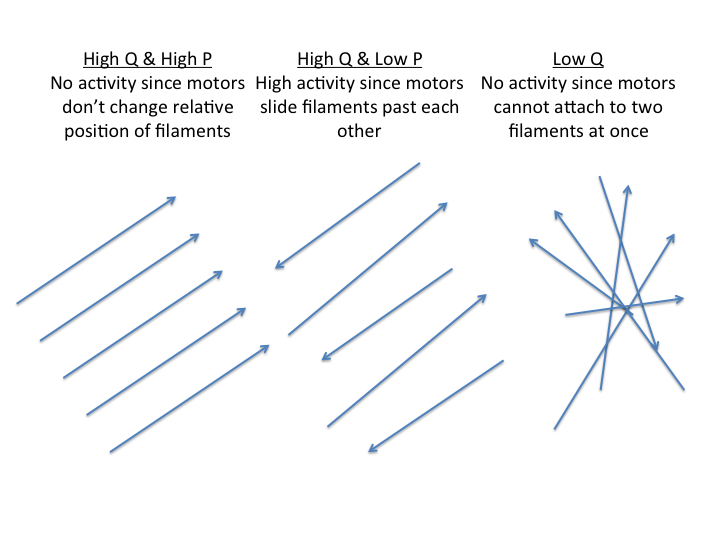
\includegraphics[width=.75\textwidth] {activity_dependence_on_QP.png}
\caption{\label{fig:activity_dependence} Read the figure...}
\end{figure}

For definiteness we will need to choose a closure relation to evaluate $<p_ip_jp_k>$.  For undisclosed reasons I'm choosing the expansion around the isotropic state where  $<p_ip_jp_k>=\frac{1}{d+2}\left(\b{P}_i\delta_{jk}+\b{P}_{j}\delta_{ik}+\b{P}_k\delta_{ij}\right)$.  The concentration again decouples so we take it to be a constant and examine the axisymmetric $\b{P,Q}$ dynamics in 2d:
\begin{gather}
\frac{\partial\b{Q}}{\partial t}=d^{(s)}\nabla_x^2(\b{Q})-4d^{(r)}\b{Q}+\frac{1}{3}\b{E\cdot Q}+\frac{2}{3}\b{Q\cdot E}-\frac{1}{3}\b{I Q:E}+\frac{1}{4}\b{E}\\
\nonumber\frac{\partial\b{P}}{\partial t}=d^{(s)}\nabla_x^2(\b{P})-d^{(r)}\b{P}+\frac{1}{2}\b{E\cdot P}\\
\nonumber\nabla\cdot(-\b{I}\Pi+2\b{E}-\sigma_0\b{Q}(1-|\b{P}|))=0,
\end{gather}
with \emph{natural} boundary conditions $\b{N}\cdot\nabla\b{Q}=0,\b{N}\cdot\nabla\b{P}=0,\b{u}=0$.  In the absence of flow ($\b{E}=0$) the equations decouple and the stationary solution has $Q=0$ for the same reasons as before. The components of $\b{P}$ satisfy
\begin{equation}
r^2\frac{\partial^2\b{P}_{\alpha}}{\partial r^2}+r \frac{\partial\b{P}_{\alpha}}{\partial r}-(1+r^2\frac{d^{(r)}}{d^{(s)}})\b{P}_{\alpha}=0,
\end{equation}
which is of the Bessel form but admits no real solutions and we thus conclude that $\b{P}=0$ in the absence of flow as well.  Now turn on $\b{E}$ and solve the stokes equation like before.  The $\hat{r}$ component again determines the pressure, while the $\hat{\theta}$ component informs us that $\b{E}_{r\theta}=\frac{\sigma_0}{2}\b{Q}_{r\theta}(1-|\b{P}|)$.  Ignore the nonlinearities while assuming somehow that $Q^2$ is higher order than $QP$ to find
\begin{gather}
\frac{\partial\b{Q}}{\partial t}=d^{(s)}\nabla_x^2(\b{Q})-4d^{(r)}\b{Q}+\frac{\sigma}{8}\b{Q}_{r\theta}(1-|\b{P}|)(\hat{r}\hat{\theta}+\hat{\theta}\hat{r})\\
\nonumber\frac{\partial\b{P}}{\partial t}=d^{(s)}\nabla_x^2(\b{P})-d^{(r)}\b{P}+\frac{\sigma}{4}\b{Q}_{r\theta}(1-|\b{P}|) (\b{P}_{\theta}\hat{r}+\b{P}_{r}\hat{\theta})
\end{gather}
Let's not worry too much about the details and instead focus on a qualitative understanding.  Starting from a no flow state I would expect $Q$ to become unstable first in the presence of sufficiently strong active stress since it is truly a linear instability.  As Q grows P will eventually become unstable and this in turn will limit the growth of Q.  As $|P|$ saturates at $1$ Q will be stabilized by the diffusive term and will start decaying until P is no longer unstable and the cycle repeats itself.  So: Nematic-Polar Oscillations in Active Suspensions. Done.  Haha.  



























\end{document}
